% !TeX program = xelatex
% 题面资源 302-question-facsimiles.pdf 与本文件放在同一目录。
\documentclass[UTF8,zihao=-4,fontset=fandol]{ctexart}
\usepackage[paperwidth=800bp,paperheight=600bp,left=52bp,right=52bp,top=42bp,bottom=47bp]{geometry}
\usepackage{amsmath,graphicx,xcolor,fancyhdr}
\usepackage[hidelinks,bookmarksopen=true]{hyperref}
\definecolor{ink}{HTML}{192635}
\definecolor{muted}{HTML}{45566A}
\definecolor{accent}{HTML}{175C57}
\setlength{\parindent}{0pt}
\setlength{\headheight}{15bp}
\pagestyle{fancy}
\fancyhf{}
\renewcommand{\headrulewidth}{0pt}
\fancyfoot[L]{\small\textcolor{muted}{\hyperlink{contents}{返回目录}}}
\fancyfoot[R]{\small\textcolor{muted}{\thepage}}
\raggedbottom
\newcommand{\SectionHeading}[4]{%
  \clearpage\hypertarget{sec-#1}{}%
  {\small\textcolor{accent}{#2\hfill 第 #1 节}}\par\medskip
  {\LARGE\bfseries #3}\par\smallskip
  {\small\textcolor{muted}{#4}}\par\bigskip}
\newcommand{\Theory}[4]{%
  {\small\textcolor{accent}{#1}\quad\textbf{#3}\hfill\textcolor{muted}{教材 PDF 第 #2 页}}\par
  {\small #4}\par\smallskip}
\newcommand{\Clip}[2]{%
  \par\nointerlineskip\hbox to \linewidth{\hfil
  \includegraphics[page=#1,width=#2bp]{302-question-facsimiles.pdf}\hfil}%
  \vspace{5bp}}
\newcommand{\QuestionPage}[7]{%
  \clearpage
  {\small\textcolor{accent}{#1\hfill #2}}\par\medskip
  {\Large\bfseries #3}\hfill {\small\textcolor{muted}{原卷 PDF 第 #4 页}}\par
  {\small\textcolor{muted}{#5\hfill #6}}\par\vspace{9bp}#7}
\begin{document}
\hypertarget{contents}{}
{\small\textcolor{accent}{302\quad 全国硕士研究生招生考试\hfill 4:3 横屏}}\par\bigskip
{\huge\bfseries 数学二分节真题集}\par\smallskip
{\large iPad 手写练习版}\par\smallskip
{\small 2009--2026 年\quad 408 题\quad 上册 19 节\qquad 点击目录进入对应小节。}\par\bigskip

\begin{minipage}[t]{0.48\linewidth}
\medskip\textbf{函数、极限、连续}\par
{\small\hyperlink{sec-1.1}{1.1\quad 集合、映射与函数}\hfill 1 题}\par
{\small\hyperlink{sec-1.2}{1.2\quad 数列的极限}\hfill 10 题}\par
{\small\hyperlink{sec-1.3}{1.3\quad 函数的极限}\hfill 5 题}\par
{\small\hyperlink{sec-1.4}{1.4\quad 无穷小量与无穷大量}\hfill 23 题}\par
{\small\hyperlink{sec-1.5}{1.5\quad 连续函数}\hfill 8 题}\par
\medskip\textbf{一元函数微分学及其应用}\par
{\small\hyperlink{sec-2.1}{2.1\quad 导数的概念}\hfill 8 题}\par
{\small\hyperlink{sec-2.2}{2.2\quad 求导的基本法则}\hfill 28 题}\par
{\small\hyperlink{sec-2.3}{2.3\quad 微分}\hfill 0 题}\par
{\small\hyperlink{sec-2.4}{2.4\quad 微分中值定理及其应用}\hfill 12 题}\par
{\small\hyperlink{sec-2.5}{2.5\quad Taylor定理及其应用}\hfill 9 题}\par
{\small\hyperlink{sec-2.6}{2.6\quad 函数性态的研究}\hfill 25 题}\par
\end{minipage}%
\hfill
\begin{minipage}[t]{0.48\linewidth}
\medskip\textbf{一元函数积分学及其应用}\par
{\small\hyperlink{sec-3.1}{3.1\quad 定积分的概念、存在条件与性质}\hfill 11 题}\par
{\small\hyperlink{sec-3.2}{3.2\quad 微积分基本公式与基本定理}\hfill 11 题}\par
{\small\hyperlink{sec-3.3}{3.3\quad 两种基本积分法}\hfill 14 题}\par
{\small\hyperlink{sec-3.4}{3.4\quad 定积分的应用}\hfill 25 题}\par
{\small\hyperlink{sec-3.5}{3.5\quad 反常积分}\hfill 13 题}\par
\medskip\textbf{常微分方程}\par
{\small\hyperlink{sec-4.1}{4.1\quad 几类简单的微分方程}\hfill 17 题}\par
{\small\hyperlink{sec-4.2}{4.2\quad 高阶线性微分方程}\hfill 16 题}\par
{\small\hyperlink{sec-4.3}{4.3\quad 线性微分方程组（教材星号节）}\hfill 0 题}\par
\medskip\textbf{上册范围外真题}\par
{\small\hyperlink{sec-A.1}{A.1\quad 多元函数微分学}\hfill 44 题}\par
{\small\hyperlink{sec-A.2}{A.2\quad 二重积分}\hfill 30 题}\par
{\small\hyperlink{sec-A.3}{A.3\quad 曲率与曲率圆}\hfill 8 题}\par
{\small\hyperlink{sec-A.4}{A.4\quad 线性代数}\hfill 90 题}\par
\end{minipage}%
\SectionHeading{1.1}{函数、极限、连续}{集合、映射与函数}{定理与要点\quad 教材 PDF 第 24 页起\hfill 本节 1 题}
\pdfbookmark[1]{函数、极限、连续}{chapter-1.1}
\pdfbookmark[2]{1.1 集合、映射与函数}{section-1.1}
\Theory{定理 1.1}{29}{确界存在定理}{非空实数集若有上界，就有上确界。若有下界，就有下确界。}
\Theory{定理 1.2}{36}{逆映射存在定理}{一一映射（双射）f 从 A 到 B 有唯一逆映射，从 B 返回 A。}
\Theory{要点}{33--36}{函数性质与复合}{奇偶性先核对定义域关于原点对称。求复合函数时，同时限制内层的定义域和外层的输入。}
\QuestionPage{1.1 集合、映射与函数}{选择题}{2024 年第 3 题}{1}{函数的奇偶性}{001 / 408}{\Clip{347}{696.000}}
\SectionHeading{1.2}{函数、极限、连续}{数列的极限}{定理与要点\quad 教材 PDF 第 41 页起\hfill 本节 10 题}
\pdfbookmark[2]{1.2 数列的极限}{section-1.2}
\Theory{定理 2.1}{46}{唯一性}{收敛数列只有一个极限。}
\Theory{定理 2.2}{47}{有界性}{收敛数列必有界。}
\Theory{定理 2.3}{47}{有理运算法则}{两收敛数列可逐项作和、差、积、商再取极限，取商时分母极限须非零。}
\Theory{定理 2.4}{49}{保号性}{数列收敛到非零值时，从某一项起与极限同号，并且绝对值离零有正的下界。}
\Theory{定理 2.5}{49}{夹逼性}{两端数列收敛到同一值时，最终被夹在其间的数列也收敛到该值。}
\Theory{定理 2.6}{51}{单调有界准则}{单调增且有上界，或单调减且有下界的数列必收敛。}
\Theory{定理 2.7}{54}{子列与极限}{数列收敛到 a，当且仅当其每个子列都收敛到 a。}
\Theory{定理 2.8}{54}{闭区间套定理}{逐级包含且长度趋于零的非空闭区间列，恰有一个公共点。}
\Theory{定理 2.9}{55}{Weierstrass 定理}{有界实数列至少有一个收敛子列。}
\Theory{定理 2.10}{56}{Cauchy 收敛原理}{实数列收敛，当且仅当任给正误差，充分靠后的任意两项之差的绝对值都小于该误差。}
\QuestionPage{1.2 数列的极限}{选择题}{2012 年第 3 题}{1}{数列与部分和的收敛}{002 / 408}{\Clip{74}{696.000}}
\QuestionPage{1.2 数列的极限}{选择题}{2017 年第 3 题}{1}{收敛数列的性质}{003 / 408}{\Clip{189}{696.000}}
\QuestionPage{1.2 数列的极限}{选择题}{2022 年第 6 题}{1}{递推数列的性质}{004 / 408}{\Clip{306}{696.000}}
\QuestionPage{1.2 数列的极限}{选择题}{2023 年第 3 题}{1}{递推数列与无穷小比较}{005 / 408}{\Clip{325}{696.000}}
\QuestionPage{1.2 数列的极限}{选择题}{2024 年第 4 题}{1}{数列极限的敛散性}{006 / 408}{\Clip{348}{696.000}}
\QuestionPage{1.2 数列的极限}{填空题}{2012 年第 10 题}{2}{和式型数列极限与夹逼准则}{007 / 408}{\Clip{81}{696.000}}
\QuestionPage{1.2 数列的极限}{解答题}{2011 年第 19 题}{3}{调和和式与数列收敛}{008 / 408}{\Clip{67}{696.000}}
\QuestionPage{1.2 数列的极限}{解答题}{2012 年第 21 题}{4}{实根构成的数列极限}{009 / 408}{\Clip{92}{696.000}}
\QuestionPage{1.2 数列的极限}{解答题}{2013 年第 20 题}{3}{不等式约束下的数列极限}{010 / 408}{\Clip{114}{696.000}}
\QuestionPage{1.2 数列的极限}{解答题}{2018 年第 21 题}{4}{递推数列的收敛与极限}{011 / 408}{\Clip{230}{696.000}}
\SectionHeading{1.3}{函数、极限、连续}{函数的极限}{定理与要点\quad 教材 PDF 第 60 页起\hfill 本节 5 题}
\pdfbookmark[2]{1.3 函数的极限}{section-1.3}
\Theory{定理 3.1}{65}{Heine 定理}{去心邻域内，函数极限等于 a，当且仅当沿任意趋于该点的数列，函数值都趋于 a。}
\Theory{定理 3.2}{66}{唯一性与局部有界性}{函数的有限极限唯一，且函数在相应去心邻域内有界。}
\Theory{定理 3.3}{67}{保号、保序和夹逼}{非零极限在局部保号。局部大小关系传给极限，两端极限相同即可夹逼。}
\Theory{定理 3.4}{67}{有理运算法则}{和、差、积的极限由各自极限运算得到。商的分母极限须非零。}
\Theory{定理 3.5}{69}{复合函数的极限}{内层趋于 u\textsubscript{0} 且在去心邻域内避开 u\textsubscript{0} 时，可应用外层在 u\textsubscript{0} 的极限。}
\Theory{定理 3.6}{73}{单调有界准则}{在右半无限区间单调增且有上界或单调减且有下界时，右端极限存在。单调函数在区间内点有左右极限。}
\Theory{定理 3.7}{74}{Cauchy 收敛原理}{有限极限存在，当且仅当充分接近目标点的任意两处函数值都可彼此任意接近。}
\Theory{公式}{70--72}{两个重要极限}{x \ensuremath{\to} 0 时 sin x / x \ensuremath{\to} 1。u \ensuremath{\to} 0 时 (1 + u)\textasciicircum{}(1/u) \ensuremath{\to} e。}
\QuestionPage{1.3 函数的极限}{填空题}{2011 年第 9 题}{1}{函数极限}{012 / 408}{\Clip{57}{696.000}}
\QuestionPage{1.3 函数的极限}{填空题}{2013 年第 9 题}{2}{指数型函数极限}{013 / 408}{\Clip{103}{696.000}}
\QuestionPage{1.3 函数的极限}{填空题}{2019 年第 9 题}{1}{指数型函数极限}{014 / 408}{\Clip{241}{696.000}}
\QuestionPage{1.3 函数的极限}{填空题}{2022 年第 11 题}{2}{指数型函数极限}{015 / 408}{\Clip{311}{696.000}}
\QuestionPage{1.3 函数的极限}{解答题}{2011 年第 15 题}{2}{两处函数极限与参数}{016 / 408}{\Clip{63}{696.000}}
\SectionHeading{1.4}{函数、极限、连续}{无穷小量与无穷大量}{定理与要点\quad 教材 PDF 第 77 页起\hfill 本节 23 题}
\pdfbookmark[2]{1.4 无穷小量与无穷大量}{section-1.4}
\Theory{定理 4.1}{78}{极限与无穷小}{f 趋于有限值 a，当且仅当 f 可写成 a 加一个无穷小。}
\Theory{定理 4.2}{78}{无穷小的和与积}{在同一变化趋势下，有限个无穷小的代数和及乘积仍为无穷小。}
\Theory{定理 4.3}{78}{有界量乘无穷小}{局部有界函数乘无穷小，结果仍为无穷小。}
\Theory{定理 4.4}{81}{等价无穷小}{两非零无穷小等价，表示两者之差相对于其中任一量为高阶无穷小。}
\Theory{定理 4.5}{82}{无穷小等价代换}{求商的极限时，分子和分母的无穷小因子可分别换成各自的等价量。}
\Theory{定理 4.6}{84}{倒数关系}{非零无穷小的倒数为无穷大量，无穷大量的倒数为无穷小。}
\Theory{定理 4.7}{84}{无穷大量的运算}{有限个无穷大量的乘积仍是无穷大量。无穷大量与有界量的和仍是无穷大量。}
\Theory{公式}{82--85}{常用等价式与渐近线}{x \ensuremath{\to} 0 时 sin x \ensuremath{\sim} x，1 \ensuremath{-} cos x \ensuremath{\sim} x\textsuperscript{2}/2。求斜渐近线可依次取 f(x)/x 和 f(x) \ensuremath{-} kx 的极限。}
\QuestionPage{1.4 无穷小量与无穷大量}{选择题}{2009 年第 2 题}{1}{等价无穷小}{017 / 408}{\Clip{2}{696.000}}
\QuestionPage{1.4 无穷小量与无穷大量}{选择题}{2011 年第 1 题}{1}{三角函数的等价无穷小}{018 / 408}{\Clip{49}{696.000}}
\QuestionPage{1.4 无穷小量与无穷大量}{选择题}{2012 年第 1 题}{1}{渐近线条数}{019 / 408}{\Clip{72}{696.000}}
\QuestionPage{1.4 无穷小量与无穷大量}{选择题}{2013 年第 1 题}{1}{三角无穷小的比较}{020 / 408}{\Clip{95}{696.000}}
\QuestionPage{1.4 无穷小量与无穷大量}{选择题}{2014 年第 1 题}{1}{幂次与无穷小阶}{021 / 408}{\Clip{118}{696.000}}
\QuestionPage{1.4 无穷小量与无穷大量}{选择题}{2014 年第 2 题}{1}{渐近线的判定}{022 / 408}{\Clip{119}{696.000}}
\QuestionPage{1.4 无穷小量与无穷大量}{选择题}{2016 年第 1 题}{1}{无穷小量的阶}{023 / 408}{\Clip{164}{696.000}}
\QuestionPage{1.4 无穷小量与无穷大量}{选择题}{2019 年第 1 题}{1}{正切函数的同阶无穷小}{024 / 408}{\Clip{233}{696.000}}
\QuestionPage{1.4 无穷小量与无穷大量}{选择题}{2020 年第 1 题}{1}{积分形式的无穷小比阶}{025 / 408}{\Clip{256}{696.000}}
\QuestionPage{1.4 无穷小量与无穷大量}{选择题}{2021 年第 1 题}{1}{变上限积分的无穷小阶}{026 / 408}{\Clip{279}{696.000}}
\QuestionPage{1.4 无穷小量与无穷大量}{选择题}{2022 年第 1 题}{1}{等价无穷小的性质}{027 / 408}{\Clip{301}{696.000}}
\QuestionPage{1.4 无穷小量与无穷大量}{选择题}{2023 年第 1 题}{1}{斜渐近线}{028 / 408}{\Clip{323}{696.000}}
\QuestionPage{1.4 无穷小量与无穷大量}{选择题}{2025 年第 4 题}{1}{无穷小比阶}{029 / 408}{\Clip{370}{696.000}}
\QuestionPage{1.4 无穷小量与无穷大量}{选择题}{2026 年第 1 题}{1}{等价无穷小求系数}{030 / 408}{\Clip{389}{696.000}}
\QuestionPage{1.4 无穷小量与无穷大量}{填空题}{2010 年第 10 题}{2}{曲线的渐近线}{031 / 408}{\Clip{35}{696.000}}
\QuestionPage{1.4 无穷小量与无穷大量}{填空题}{2016 年第 9 题}{2}{斜渐近线}{032 / 408}{\Clip{172}{696.000}}
\QuestionPage{1.4 无穷小量与无穷大量}{填空题}{2017 年第 9 题}{2}{斜渐近线}{033 / 408}{\Clip{195}{696.000}}
\QuestionPage{1.4 无穷小量与无穷大量}{填空题}{2023 年第 11 题}{2}{等价无穷小求系数}{034 / 408}{\Clip{333}{696.000}}
\QuestionPage{1.4 无穷小量与无穷大量}{填空题}{2025 年第 12 题}{2}{斜渐近线}{035 / 408}{\Clip{378}{696.000}}
\QuestionPage{1.4 无穷小量与无穷大量}{解答题}{2012 年第 15 题}{2}{同阶无穷小与参数}{036 / 408}{\Clip{86}{696.000}}
\QuestionPage{1.4 无穷小量与无穷大量}{解答题}{2013 年第 15 题}{2}{三角乘积的等价无穷小}{037 / 408}{\Clip{109}{696.000}}
\QuestionPage{1.4 无穷小量与无穷大量}{解答题}{2015 年第 15 题}{2}{等价无穷小求参数}{038 / 408}{\Clip{155}{696.000}}
\QuestionPage{1.4 无穷小量与无穷大量}{解答题}{2020 年第 15 题}{2}{斜渐近线}{039 / 408}{\Clip{270}{696.000}}
\SectionHeading{1.5}{函数、极限、连续}{连续函数}{定理与要点\quad 教材 PDF 第 86 页起\hfill 本节 8 题}
\pdfbookmark[2]{1.5 连续函数}{section-1.5}
\Theory{定理 5.1}{90}{连续函数的四则运算}{在同一点连续的函数，其和、差、积、商仍连续，取商时分母在该点非零。}
\Theory{定理 5.2}{90}{复合函数的连续性}{内层在 x\textsubscript{0} 连续，外层在内层对应值连续，则复合函数在 x\textsubscript{0} 连续。}
\Theory{定理 5.3}{91}{反函数的连续性}{区间上的连续严格单调函数有反函数，且反函数在值域上连续并保持单调方向。}
\Theory{定理 5.4}{94}{有界性}{闭区间上的连续函数有界。}
\Theory{定理 5.5}{94}{最大最小值定理}{闭区间上的连续函数能取到最大值和最小值。}
\Theory{定理 5.6}{95}{零点存在定理}{闭区间上连续且两端值异号，区间内部至少有一处零点。}
\Theory{定理 5.7}{97}{介值定理}{闭区间上的连续函数取到介于端点函数值之间的每一个值。}
\Theory{定理 5.8}{100}{一致连续性}{闭区间上的连续函数一致连续。}
\Theory{定理 5.9}{101}{压缩映射原理（星号内容）}{实直线上的压缩映射有唯一不动点，从任意实数开始迭代均收敛到该点。}
\Theory{要点}{86--89}{间断点分类}{先检查两侧极限是否有限且相等，再将共同极限与函数值比较。}
\QuestionPage{1.5 连续函数}{选择题}{2009 年第 1 题}{1}{可去间断点}{040 / 408}{\Clip{1}{696.000}}
\QuestionPage{1.5 连续函数}{选择题}{2010 年第 1 题}{1}{无穷间断点}{041 / 408}{\Clip{25}{696.000}}
\QuestionPage{1.5 连续函数}{选择题}{2015 年第 2 题}{1}{由极限定义的函数及间断点}{042 / 408}{\Clip{142}{696.000}}
\QuestionPage{1.5 连续函数}{选择题}{2015 年第 3 题}{1}{分段函数连续性与参数}{043 / 408}{\Clip{143}{696.000}}
\QuestionPage{1.5 连续函数}{选择题}{2017 年第 1 题}{1}{分段函数的连续条件}{044 / 408}{\Clip{187}{696.000}}
\QuestionPage{1.5 连续函数}{选择题}{2018 年第 3 题}{1}{分段函数和的连续性}{045 / 408}{\Clip{212}{696.000}}
\QuestionPage{1.5 连续函数}{选择题}{2020 年第 2 题}{1}{第二类间断点}{046 / 408}{\Clip{257}{696.000}}
\QuestionPage{1.5 连续函数}{选择题}{2024 年第 1 题}{1}{间断点个数}{047 / 408}{\Clip{345}{696.000}}
\SectionHeading{2.1}{一元函数微分学及其应用}{导数的概念}{定理与要点\quad 教材 PDF 第 108 页起\hfill 本节 8 题}
\pdfbookmark[1]{一元函数微分学及其应用}{chapter-2.1}
\pdfbookmark[2]{2.1 导数的概念}{section-2.1}
\Theory{定理 1.1}{115}{可导推出连续}{函数在某点可导，则在该点连续。}
\Theory{要点}{108--115}{导数定义与几何意义}{差商的左右极限须存在且相等。有限导数给出切线斜率，非零时法线斜率为其负倒数。}
\QuestionPage{2.1 导数的概念}{选择题}{2010 年第 3 题}{1}{曲线相切}{048 / 408}{\Clip{27}{696.000}}
\QuestionPage{2.1 导数的概念}{选择题}{2011 年第 2 题}{1}{导数定义与极限}{049 / 408}{\Clip{50}{696.000}}
\QuestionPage{2.1 导数的概念}{选择题}{2018 年第 2 题}{1}{原点处的可导性}{050 / 408}{\Clip{211}{696.000}}
\QuestionPage{2.1 导数的概念}{选择题}{2021 年第 2 题}{1}{分段函数的可导性与极值}{051 / 408}{\Clip{280}{696.000}}
\QuestionPage{2.1 导数的概念}{选择题}{2025 年第 7 题}{2}{可导的等价条件}{052 / 408}{\Clip{373}{696.000}}
\QuestionPage{2.1 导数的概念}{填空题}{2009 年第 9 题}{2}{切线方程}{053 / 408}{\Clip{10}{696.000}}
\QuestionPage{2.1 导数的概念}{解答题}{2022 年第 17 题}{2}{由极限求导数}{054 / 408}{\Clip{317}{696.000}}
\QuestionPage{2.1 导数的概念}{解答题}{2025 年第 18 题}{3}{由极限判断可导性}{055 / 408}{\Clip{384}{696.000}}
\SectionHeading{2.2}{一元函数微分学及其应用}{求导的基本法则}{定理与要点\quad 教材 PDF 第 121 页起\hfill 本节 28 题}
\pdfbookmark[2]{2.2 求导的基本法则}{section-2.2}
\Theory{定理 2.1}{121}{导数的有理运算法则}{可导函数的和、差、积、商可导。乘积用乘积法则，商须分母非零。}
\Theory{定理 2.2}{123}{链式法则}{内外两层在相应点可导时，复合函数的导数等于外层导数乘内层导数。}
\Theory{定理 2.3}{125}{反函数求导法则}{严格单调连续函数在对应点可导且导数非零时，反函数导数等于原导数的倒数。}
\Theory{定理 2.4}{130}{高阶导数的运算}{n 阶导数满足线性法则。乘积的 n 阶导数按 Leibniz 公式作二项式系数加权求和。}
\Theory{定理 2.5}{132}{参数方程求导法则}{当 x\ensuremath{{}^{\prime}}(t) 非零时，dy/dx = y\ensuremath{{}^{\prime}}(t)/x\ensuremath{{}^{\prime}}(t)。再对 t 求导并除以 x\ensuremath{{}^{\prime}}(t) 得二阶导数。}
\Theory{方法}{130--135}{隐函数与相关变化率}{先按变量依赖关系求导，再代入给定点或时刻。隐函数项需乘上相应的导数。}
\QuestionPage{2.2 求导的基本法则}{选择题}{2012 年第 2 题}{1}{乘积求导}{056 / 408}{\Clip{73}{696.000}}
\QuestionPage{2.2 求导的基本法则}{选择题}{2013 年第 2 题}{1}{隐函数求导与极限}{057 / 408}{\Clip{96}{696.000}}
\QuestionPage{2.2 求导的基本法则}{选择题}{2021 年第 3 题}{1}{圆柱体的相关变化率}{058 / 408}{\Clip{281}{696.000}}
\QuestionPage{2.2 求导的基本法则}{选择题}{2023 年第 5 题}{1}{隐函数求导}{059 / 408}{\Clip{327}{696.000}}
\QuestionPage{2.2 求导的基本法则}{选择题}{2024 年第 2 题}{1}{参数方程求导与导数定义}{060 / 408}{\Clip{346}{696.000}}
\QuestionPage{2.2 求导的基本法则}{选择题}{2026 年第 6 题}{1}{反函数与变上限积分求导}{061 / 408}{\Clip{394}{696.000}}
\QuestionPage{2.2 求导的基本法则}{填空题}{2009 年第 12 题}{2}{隐函数求导}{062 / 408}{\Clip{13}{696.000}}
\QuestionPage{2.2 求导的基本法则}{填空题}{2010 年第 11 题}{2}{对数函数的高阶导数}{063 / 408}{\Clip{36}{696.000}}
\QuestionPage{2.2 求导的基本法则}{填空题}{2010 年第 13 题}{2}{相关变化率}{064 / 408}{\Clip{38}{696.000}}
\QuestionPage{2.2 求导的基本法则}{填空题}{2012 年第 9 题}{2}{隐函数求导}{065 / 408}{\Clip{80}{696.000}}
\QuestionPage{2.2 求导的基本法则}{填空题}{2013 年第 10 题}{2}{反函数求导}{066 / 408}{\Clip{104}{696.000}}
\QuestionPage{2.2 求导的基本法则}{填空题}{2013 年第 12 题}{2}{参数曲线的法线}{067 / 408}{\Clip{106}{696.000}}
\QuestionPage{2.2 求导的基本法则}{填空题}{2014 年第 10 题}{2}{奇偶性、周期性与求导}{068 / 408}{\Clip{127}{696.000}}
\QuestionPage{2.2 求导的基本法则}{填空题}{2014 年第 12 题}{2}{极坐标曲线的切线}{069 / 408}{\Clip{129}{696.000}}
\QuestionPage{2.2 求导的基本法则}{填空题}{2015 年第 9 题}{2}{隐函数求导}{070 / 408}{\Clip{149}{696.000}}
\QuestionPage{2.2 求导的基本法则}{填空题}{2015 年第 10 题}{2}{高阶导数}{071 / 408}{\Clip{150}{696.000}}
\QuestionPage{2.2 求导的基本法则}{填空题}{2016 年第 13 题}{2}{动点距离的相关变化率}{072 / 408}{\Clip{176}{696.000}}
\QuestionPage{2.2 求导的基本法则}{填空题}{2017 年第 10 题}{2}{参数方程求导}{073 / 408}{\Clip{196}{696.000}}
\QuestionPage{2.2 求导的基本法则}{填空题}{2019 年第 10 题}{1}{参数曲线切线的截距}{074 / 408}{\Clip{242}{696.000}}
\QuestionPage{2.2 求导的基本法则}{填空题}{2019 年第 13 题}{2}{高阶导数}{075 / 408}{\Clip{245}{696.000}}
\QuestionPage{2.2 求导的基本法则}{填空题}{2020 年第 9 题}{2}{参数方程的导数}{076 / 408}{\Clip{264}{696.000}}
\QuestionPage{2.2 求导的基本法则}{填空题}{2021 年第 12 题}{2}{参数方程求导}{077 / 408}{\Clip{290}{696.000}}
\QuestionPage{2.2 求导的基本法则}{填空题}{2022 年第 12 题}{2}{隐函数的二阶导数}{078 / 408}{\Clip{312}{696.000}}
\QuestionPage{2.2 求导的基本法则}{填空题}{2023 年第 14 题}{2}{隐函数曲线的法线}{079 / 408}{\Clip{336}{696.000}}
\QuestionPage{2.2 求导的基本法则}{填空题}{2024 年第 14 题}{2}{高阶导数}{080 / 408}{\Clip{358}{696.000}}
\QuestionPage{2.2 求导的基本法则}{填空题}{2025 年第 14 题}{2}{隐函数与参数方程求导}{081 / 408}{\Clip{380}{696.000}}
\QuestionPage{2.2 求导的基本法则}{解答题}{2010 年第 17 题}{3}{参数方程的二阶导数}{082 / 408}{\Clip{42}{696.000}}
\QuestionPage{2.2 求导的基本法则}{解答题}{2018 年第 20 题}{3}{面积的相关变化率}{083 / 408}{\Clip{229}{696.000}}
\SectionHeading{2.3}{一元函数微分学及其应用}{微分}{定理与要点\quad 教材 PDF 第 140 页起\hfill 本节 0 题}
\pdfbookmark[2]{2.3 微分}{section-2.3}
\Theory{定理 3.1}{141}{可微与可导的等价性}{一元函数在一点可微当且仅当在该点可导，此时 df = f\ensuremath{{}^{\prime}}(x) dx。}
\Theory{公式}{143--144}{微分及线性近似}{一阶微分形式适用于复合变量。在增量足够小时，用 f\ensuremath{{}^{\prime}}(x) dx 近似函数增量。}
本节在所收原卷中没有以该节为主考点的题目。
\SectionHeading{2.4}{一元函数微分学及其应用}{微分中值定理及其应用}{定理与要点\quad 教材 PDF 第 147 页起\hfill 本节 12 题}
\pdfbookmark[2]{2.4 微分中值定理及其应用}{section-2.4}
\Theory{定理 4.1}{147}{Fermat 定理}{内点取得局部极值且在该点可导，则导数为零。}
\Theory{定理 4.2}{148}{Rolle 定理}{闭区间上连续、开区间内可导且端点值相等，内部存在导数为零的点。}
\Theory{定理 4.3}{150}{Lagrange 中值定理}{闭区间上连续、开区间内可导，内部存在一点，其导数等于全区间的平均变化率。}
\Theory{定理 4.4}{154}{Cauchy 中值定理}{两函数闭区间上连续、开区间内可导，且 g\ensuremath{{}^{\prime}} 恒非零。内部某点的导数比等于端点增量比。}
\Theory{定理 4.5}{154--155}{洛必达法则，0/0 型}{两函数趋零，邻域内可导且分母导数非零。若导数之比有极限，则原商有同一极限。}
\Theory{定理 4.6}{156}{洛必达法则，\ensuremath{\infty}/\ensuremath{\infty} 型}{两函数在同一变化趋势下为无穷大量，其余条件沿用定理 4.5，可由导数比求原商极限。}
\Theory{推论 4.3}{152}{端点导数}{函数在端点连续、在相邻开区间可导且导数的单侧极限有限时，该极限就是端点的单侧导数。}
\QuestionPage{2.4 微分中值定理及其应用}{选择题}{2014 年第 5 题}{1}{洛必达法则与函数极限}{084 / 408}{\Clip{122}{696.000}}
\QuestionPage{2.4 微分中值定理及其应用}{选择题}{2017 年第 2 题}{1}{由可导条件推断中值点}{085 / 408}{\Clip{188}{696.000}}
\QuestionPage{2.4 微分中值定理及其应用}{填空题}{2018 年第 9 题}{2}{反正切差的极限与中值定理}{086 / 408}{\Clip{218}{696.000}}
\QuestionPage{2.4 微分中值定理及其应用}{解答题}{2009 年第 21 题}{4}{拉格朗日中值定理}{087 / 408}{\Clip{22}{696.000}}
\QuestionPage{2.4 微分中值定理及其应用}{解答题}{2010 年第 21 题}{4}{两段区间上的中值定理}{088 / 408}{\Clip{46}{696.000}}
\QuestionPage{2.4 微分中值定理及其应用}{解答题}{2013 年第 18 题}{3}{奇函数与中值定理}{089 / 408}{\Clip{112}{696.000}}
\QuestionPage{2.4 微分中值定理及其应用}{解答题}{2015 年第 21 题}{4}{切线与中值定理证明}{090 / 408}{\Clip{161}{696.000}}
\QuestionPage{2.4 微分中值定理及其应用}{解答题}{2017 年第 15 题}{2}{变上限积分的未定式极限}{091 / 408}{\Clip{201}{696.000}}
\QuestionPage{2.4 微分中值定理及其应用}{解答题}{2017 年第 19 题}{3}{罗尔定理与方程的根}{092 / 408}{\Clip{205}{696.000}}
\QuestionPage{2.4 微分中值定理及其应用}{解答题}{2019 年第 21 题}{4}{中值定理与导数估计}{093 / 408}{\Clip{253}{696.000}}
\QuestionPage{2.4 微分中值定理及其应用}{解答题}{2023 年第 21 题}{4}{极值条件与二阶中值结论}{094 / 408}{\Clip{343}{696.000}}
\QuestionPage{2.4 微分中值定理及其应用}{解答题}{2024 年第 21 题}{3}{中值定理与导数估计}{095 / 408}{\Clip{365}{696.000}}
\SectionHeading{2.5}{一元函数微分学及其应用}{Taylor定理及其应用}{定理与要点\quad 教材 PDF 第 161 页起\hfill 本节 9 题}
\pdfbookmark[2]{2.5 Taylor定理及其应用}{section-2.5}
\Theory{定理 5.1}{162}{带 Peano 余项的 Taylor 定理}{若 f 在 x\textsubscript{0} 处 n 阶可微，函数等于该点 n 次 Taylor 多项式加 o((x \ensuremath{-} x\textsubscript{0})\textasciicircum{}n)。}
\Theory{定理 5.2}{164}{带 Lagrange 余项的 Taylor 定理}{区间上 n+1 阶可导时，余项为 f\textasciicircum{}(n+1)(\ensuremath{\xi})(x \ensuremath{-} x\textsubscript{0})\textasciicircum{}(n+1)/(n+1)!，\ensuremath{\xi} 在两点之间。}
\Theory{公式}{165--167}{Maclaurin 公式}{在 x = 0 处展开时，n 次项的系数为 f\textasciicircum{}(n)(0)/n!。求极限时保留到相消后首个非零项。}
\QuestionPage{2.5 Taylor定理及其应用}{选择题}{2018 年第 1 题}{1}{指数型极限与展开}{096 / 408}{\Clip{210}{696.000}}
\QuestionPage{2.5 Taylor定理及其应用}{选择题}{2020 年第 4 题}{1}{由幂级展开求高阶导数值}{097 / 408}{\Clip{259}{696.000}}
\QuestionPage{2.5 Taylor定理及其应用}{选择题}{2021 年第 5 题}{1}{二次泰勒多项式}{098 / 408}{\Clip{283}{696.000}}
\QuestionPage{2.5 Taylor定理及其应用}{选择题}{2022 年第 3 题}{1}{二阶展开与极限}{099 / 408}{\Clip{303}{696.000}}
\QuestionPage{2.5 Taylor定理及其应用}{填空题}{2026 年第 12 题}{2}{局部展开求函数极限}{100 / 408}{\Clip{400}{696.000}}
\QuestionPage{2.5 Taylor定理及其应用}{解答题}{2009 年第 15 题}{3}{展开求极限}{101 / 408}{\Clip{16}{696.000}}
\QuestionPage{2.5 Taylor定理及其应用}{解答题}{2014 年第 15 题}{2}{变上限积分与局部展开}{102 / 408}{\Clip{132}{696.000}}
\QuestionPage{2.5 Taylor定理及其应用}{解答题}{2016 年第 15 题}{2}{三角函数展开求极限}{103 / 408}{\Clip{178}{696.000}}
\QuestionPage{2.5 Taylor定理及其应用}{解答题}{2021 年第 17 题}{2}{局部展开求极限}{104 / 408}{\Clip{295}{696.000}}
\SectionHeading{2.6}{一元函数微分学及其应用}{函数性态的研究}{定理与要点\quad 教材 PDF 第 171 页起\hfill 本节 25 题}
\pdfbookmark[2]{2.6 函数性态的研究}{section-2.6}
\Theory{定理 6.1}{171}{单调性判别}{区间上连续且内部可导，单调增（减）等价于内部导数非负（非正）。严格正（负）可推出严格单调。}
\Theory{定理 6.2}{173}{极值的第一判别法}{驻点左侧导数非负、右侧非正时为极大值，反向为极小值。两侧导数严格同号时无极值。}
\Theory{定理 6.3}{174}{极值的第二判别法}{驻点处二阶导数为正则取极小值，为负则取极大值。}
\Theory{定理 6.4}{175}{高阶导数判别极值}{驻点的首个非零高阶导数若为偶数阶，正值对应极小、负值对应极大。奇数阶无极值。}
\Theory{定理 6.5}{179}{凹凸性判别}{按本书术语，区间内 f\ensuremath{{}^{\prime\prime}} > 0 则图像为凹，f\ensuremath{{}^{\prime\prime}} < 0 则为凸。}
\Theory{要点}{175--182}{最值与拐点}{闭区间求最值要比较内部候选点和端点。判定拐点要核对曲线两侧凹凸性变化。}
\QuestionPage{2.6 函数性态的研究}{选择题}{2011 年第 3 题}{1}{驻点个数}{105 / 408}{\Clip{51}{696.000}}
\QuestionPage{2.6 函数性态的研究}{选择题}{2014 年第 3 题}{1}{凹凸性与弦线}{106 / 408}{\Clip{120}{696.000}}
\QuestionPage{2.6 函数性态的研究}{选择题}{2015 年第 4 题}{1}{由二阶导数图像判定拐点}{107 / 408}{\Clip{144}{696.000}}
\QuestionPage{2.6 函数性态的研究}{选择题}{2016 年第 4 题}{1}{由导函数图像判断性态}{108 / 408}{\Clip{167}{696.000}}
\QuestionPage{2.6 函数性态的研究}{选择题}{2018 年第 4 题}{1}{凹凸性与积分平均值}{109 / 408}{\Clip{213}{696.000}}
\QuestionPage{2.6 函数性态的研究}{选择题}{2019 年第 2 题}{1}{拐点坐标}{110 / 408}{\Clip{234}{696.000}}
\QuestionPage{2.6 函数性态的研究}{选择题}{2020 年第 6 题}{1}{由导数不等式判断函数比值}{111 / 408}{\Clip{261}{696.000}}
\QuestionPage{2.6 函数性态的研究}{选择题}{2021 年第 4 题}{1}{单调性与零点个数}{112 / 408}{\Clip{282}{696.000}}
\QuestionPage{2.6 函数性态的研究}{选择题}{2023 年第 6 题}{1}{积分函数的最小值}{113 / 408}{\Clip{328}{696.000}}
\QuestionPage{2.6 函数性态的研究}{选择题}{2023 年第 7 题}{2}{极值点与拐点的参数条件}{114 / 408}{\Clip{329}{696.000}}
\QuestionPage{2.6 函数性态的研究}{选择题}{2025 年第 2 题}{1}{极值点和拐点的定义}{115 / 408}{\Clip{368}{696.000}}
\QuestionPage{2.6 函数性态的研究}{选择题}{2026 年第 5 题}{1}{单调性、极值与凹凸性}{116 / 408}{\Clip{393}{696.000}}
\QuestionPage{2.6 函数性态的研究}{填空题}{2009 年第 13 题}{2}{区间最值}{117 / 408}{\Clip{14}{696.000}}
\QuestionPage{2.6 函数性态的研究}{填空题}{2018 年第 10 题}{2}{拐点及其切线}{118 / 408}{\Clip{219}{696.000}}
\QuestionPage{2.6 函数性态的研究}{解答题}{2010 年第 15 题}{2}{变上限积分的单调性与极值}{119 / 408}{\Clip{40}{696.000}}
\QuestionPage{2.6 函数性态的研究}{解答题}{2011 年第 16 题}{2}{参数曲线的极值和拐点}{120 / 408}{\Clip{64}{696.000}}
\QuestionPage{2.6 函数性态的研究}{解答题}{2012 年第 20 题}{3}{用函数性态证明不等式}{121 / 408}{\Clip{91}{696.000}}
\QuestionPage{2.6 函数性态的研究}{解答题}{2015 年第 19 题}{3}{函数零点的个数}{122 / 408}{\Clip{159}{696.000}}
\QuestionPage{2.6 函数性态的研究}{解答题}{2016 年第 16 题}{2}{含绝对值的积分与最小值}{123 / 408}{\Clip{179}{696.000}}
\QuestionPage{2.6 函数性态的研究}{解答题}{2017 年第 18 题}{3}{隐函数的极值}{124 / 408}{\Clip{204}{696.000}}
\QuestionPage{2.6 函数性态的研究}{解答题}{2018 年第 18 题}{3}{构造函数证明不等式}{125 / 408}{\Clip{227}{696.000}}
\QuestionPage{2.6 函数性态的研究}{解答题}{2019 年第 15 题}{2}{求导与函数极值}{126 / 408}{\Clip{247}{696.000}}
\QuestionPage{2.6 函数性态的研究}{解答题}{2021 年第 18 题}{3}{凹凸区间与渐近线}{127 / 408}{\Clip{296}{691.908}}
\QuestionPage{2.6 函数性态的研究}{解答题}{2022 年第 21 题}{4}{二阶导数与凹凸性}{128 / 408}{\Clip{321}{696.000}}
\QuestionPage{2.6 函数性态的研究}{解答题}{2025 年第 21 题}{3}{导函数单调与函数凹凸性}{129 / 408}{\Clip{387}{696.000}}
\SectionHeading{3.1}{一元函数积分学及其应用}{定积分的概念、存在条件与性质}{定理与要点\quad 教材 PDF 第 189 页起\hfill 本节 11 题}
\pdfbookmark[1]{一元函数积分学及其应用}{chapter-3.1}
\pdfbookmark[2]{3.1 定积分的概念、存在条件与性质}{section-3.1}
\Theory{定理 1.1}{195}{可积的充要条件}{有界函数可积，当且仅当分割足够细时，各小区间的振幅乘区间长度之和可任意小。}
\Theory{定理 1.2}{196}{连续函数可积}{闭区间上的连续函数黎曼可积。}
\Theory{定理 1.3}{196}{有限间断点及单调情形}{有界函数若只有有限个第一类间断点，或在闭区间上单调，则可积。}
\Theory{性质 1.1--1.5}{197--199}{定积分的性质}{积分具有线性、保序、绝对值估计和区间可加性。可积函数的乘积仍可积。}
\Theory{性质 1.6}{199}{积分中值定理}{f 连续、g 可积且不变号，则存在 \ensuremath{\xi}，使 \ensuremath{\int} f g = f(\ensuremath{\xi}) \ensuremath{\int} g。}
\Theory{推论 1.2}{200}{积分平均值}{取权函数恒为 1，连续函数的积分平均值等于该闭区间某一点的函数值。}
\Theory{方法}{192--195}{从和式识别定积分}{把和式写成取样函数值乘小区间长度，再找分割的区间和取样点。}
\QuestionPage{3.1 定积分的概念、存在条件与性质}{选择题}{2012 年第 4 题}{1}{定积分比较}{130 / 408}{\Clip{75}{696.000}}
\QuestionPage{3.1 定积分的概念、存在条件与性质}{选择题}{2018 年第 5 题}{1}{定积分估计与比较}{131 / 408}{\Clip{214}{696.000}}
\QuestionPage{3.1 定积分的概念、存在条件与性质}{选择题}{2021 年第 7 题}{1}{定积分与黎曼和}{132 / 408}{\Clip{285}{696.000}}
\QuestionPage{3.1 定积分的概念、存在条件与性质}{选择题}{2022 年第 7 题}{2}{比较定积分大小}{133 / 408}{\Clip{307}{696.000}}
\QuestionPage{3.1 定积分的概念、存在条件与性质}{填空题}{2016 年第 10 题}{2}{三角和式极限}{134 / 408}{\Clip{173}{696.000}}
\QuestionPage{3.1 定积分的概念、存在条件与性质}{填空题}{2024 年第 15 题}{2}{速度的积分平均值}{135 / 408}{\Clip{359}{696.000}}
\QuestionPage{3.1 定积分的概念、存在条件与性质}{填空题}{2025 年第 13 题}{2}{和式极限与定积分定义}{136 / 408}{\Clip{379}{696.000}}
\QuestionPage{3.1 定积分的概念、存在条件与性质}{填空题}{2026 年第 15 题}{2}{函数的积分平均值}{137 / 408}{\Clip{403}{696.000}}
\QuestionPage{3.1 定积分的概念、存在条件与性质}{解答题}{2010 年第 16 题}{2}{积分比较与数列极限}{138 / 408}{\Clip{41}{696.000}}
\QuestionPage{3.1 定积分的概念、存在条件与性质}{解答题}{2014 年第 19 题}{3}{定积分保序与比较}{139 / 408}{\Clip{136}{696.000}}
\QuestionPage{3.1 定积分的概念、存在条件与性质}{解答题}{2020 年第 20 题}{3}{积分中值定理}{140 / 408}{\Clip{275}{696.000}}
\SectionHeading{3.2}{一元函数积分学及其应用}{微积分基本公式与基本定理}{定理与要点\quad 教材 PDF 第 203 页起\hfill 本节 11 题}
\pdfbookmark[2]{3.2 微积分基本公式与基本定理}{section-3.2}
\Theory{定理 2.1}{204}{Newton--Leibniz 公式}{可积函数在区间上有原函数 F 时，定积分等于 F(上限) \ensuremath{-} F(下限)。}
\Theory{定理 2.2}{206}{微积分第一基本定理}{连续函数的变上限积分可导，其导数等于被积函数在上限的值。}
\Theory{定理 2.3}{207}{微积分第二基本定理}{已知 f 的一个原函数 F，其全部原函数为 F + C，C 是任意常数。}
\Theory{推论 2.1}{206}{连续函数的原函数}{连续函数有原函数，固定下限的变上限积分就是其中一个。}
\Theory{公式}{206--207}{上下限均变动}{上限贡献取正，下限贡献取负，各自用被积函数值乘对应端点的导数。}
\QuestionPage{3.2 微积分基本公式与基本定理}{选择题}{2009 年第 6 题}{1、2}{变上限积分的图像}{141 / 408}{\Clip{6}{382.815}\Clip{7}{382.815}}
\QuestionPage{3.2 微积分基本公式与基本定理}{选择题}{2013 年第 3 题}{1}{变上限积分的连续性与可导性}{142 / 408}{\Clip{97}{696.000}}
\QuestionPage{3.2 微积分基本公式与基本定理}{选择题}{2016 年第 2 题}{1}{分段函数的原函数}{143 / 408}{\Clip{165}{696.000}}
\QuestionPage{3.2 微积分基本公式与基本定理}{选择题}{2023 年第 2 题}{1}{分段函数的原函数}{144 / 408}{\Clip{324}{547.813}}
\QuestionPage{3.2 微积分基本公式与基本定理}{填空题}{2015 年第 11 题}{2}{变上限积分求导}{145 / 408}{\Clip{151}{696.000}}
\QuestionPage{3.2 微积分基本公式与基本定理}{填空题}{2016 年第 12 题}{2}{变上限积分与高阶导数}{146 / 408}{\Clip{175}{696.000}}
\QuestionPage{3.2 微积分基本公式与基本定理}{填空题}{2023 年第 15 题}{2}{积分关系求函数值}{147 / 408}{\Clip{337}{696.000}}
\QuestionPage{3.2 微积分基本公式与基本定理}{解答题}{2016 年第 21 题}{4}{原函数、平均值与零点}{148 / 408}{\Clip{184}{696.000}}
\QuestionPage{3.2 微积分基本公式与基本定理}{解答题}{2018 年第 16 题}{2}{变上限积分与平均值}{149 / 408}{\Clip{225}{696.000}}
\QuestionPage{3.2 微积分基本公式与基本定理}{解答题}{2020 年第 16 题}{2}{变上限积分求导与连续性}{150 / 408}{\Clip{271}{696.000}}
\QuestionPage{3.2 微积分基本公式与基本定理}{解答题}{2026 年第 18 题}{2}{变上限积分的导数与连续性}{151 / 408}{\Clip{406}{696.000}}
\SectionHeading{3.3}{一元函数积分学及其应用}{两种基本积分法}{定理与要点\quad 教材 PDF 第 214 页起\hfill 本节 14 题}
\pdfbookmark[2]{3.3 两种基本积分法}{section-3.3}
\Theory{定理 3.1}{214}{不定积分换元法则 I}{辨认 f(\ensuremath{\varphi}(x))\ensuremath{\varphi}\ensuremath{{}^{\prime}}(x) 后，令 u = \ensuremath{\varphi}(x)，积分结果代回 u。}
\Theory{定理 3.2}{219}{不定积分换元法则 II}{令 x = \ensuremath{\varphi}(t)，在 \ensuremath{\varphi}\ensuremath{{}^{\prime}} 定号且可反解的区间内，将被积式化为 f(\ensuremath{\varphi}(t))\ensuremath{\varphi}\ensuremath{{}^{\prime}}(t) dt。}
\Theory{定理 3.3}{222}{定积分换元}{连续被积函数和连续可导换元满足教材的区间条件时，上下限随代换改变，微分乘以导数。}
\Theory{公式}{225、229}{分部积分}{\ensuremath{\int} u dv = uv \ensuremath{-} \ensuremath{\int} v du。定积分中的 uv 取两端的差。}
\QuestionPage{3.3 两种基本积分法}{选择题}{2011 年第 6 题}{1}{定积分的对称换元}{152 / 408}{\Clip{54}{696.000}}
\QuestionPage{3.3 两种基本积分法}{选择题}{2020 年第 3 题}{1}{反三角函数的换元积分}{153 / 408}{\Clip{258}{696.000}}
\QuestionPage{3.3 两种基本积分法}{选择题}{2022 年第 2 题}{1}{定积分计算}{154 / 408}{\Clip{302}{696.000}}
\QuestionPage{3.3 两种基本积分法}{填空题}{2009 年第 11 题}{2}{含参数积分与分部积分}{155 / 408}{\Clip{12}{696.000}}
\QuestionPage{3.3 两种基本积分法}{填空题}{2017 年第 11 题}{2}{定积分计算}{156 / 408}{\Clip{197}{696.000}}
\QuestionPage{3.3 两种基本积分法}{填空题}{2017 年第 13 题}{2}{三角函数的定积分}{157 / 408}{\Clip{199}{696.000}}
\QuestionPage{3.3 两种基本积分法}{填空题}{2018 年第 11 题}{2}{有理函数的积分}{158 / 408}{\Clip{220}{696.000}}
\QuestionPage{3.3 两种基本积分法}{填空题}{2020 年第 10 题}{2}{换元计算定积分}{159 / 408}{\Clip{265}{696.000}}
\QuestionPage{3.3 两种基本积分法}{填空题}{2022 年第 13 题}{2}{有理函数的定积分}{160 / 408}{\Clip{313}{696.000}}
\QuestionPage{3.3 两种基本积分法}{解答题}{2009 年第 16 题}{3}{对数函数的不定积分}{161 / 408}{\Clip{17}{696.000}}
\QuestionPage{3.3 两种基本积分法}{解答题}{2017 年第 17 题}{3}{不定积分计算}{162 / 408}{\Clip{203}{696.000}}
\QuestionPage{3.3 两种基本积分法}{解答题}{2018 年第 15 题}{2}{换元与分部积分}{163 / 408}{\Clip{224}{696.000}}
\QuestionPage{3.3 两种基本积分法}{解答题}{2019 年第 16 题}{2}{不定积分计算}{164 / 408}{\Clip{248}{696.000}}
\QuestionPage{3.3 两种基本积分法}{解答题}{2025 年第 17 题}{3}{定积分计算}{165 / 408}{\Clip{383}{696.000}}
\SectionHeading{3.4}{一元函数积分学及其应用}{定积分的应用}{定理与要点\quad 教材 PDF 第 233 页起\hfill 本节 25 题}
\pdfbookmark[2]{3.4 定积分的应用}{section-3.4}
\Theory{方法}{234--235}{微元法}{选择积分变量，把一个小区间的贡献写成主部 dQ，再对整个区间积分。}
\Theory{公式}{235--237}{平面面积}{直角坐标用上、下边界的差积分。极坐标扇形面积微元为 \ensuremath{\rho}\textsuperscript{2} d\ensuremath{\theta}/2。}
\Theory{公式}{237--239}{旋转体积}{截面积沿轴积分。圆柱壳法用周长乘壳高再乘厚度。}
\Theory{方法}{239--242}{物理应用}{以薄层或小段建立功、压力等贡献的微元，并保留单位和力的作用方向。}
\QuestionPage{3.4 定积分的应用}{选择题}{2017 年第 6 题}{1}{速度图像与追及距离}{166 / 408}{\Clip{192}{696.000}}
\QuestionPage{3.4 定积分的应用}{选择题}{2025 年第 6 题}{1}{克服引力做功}{167 / 408}{\Clip{372}{696.000}}
\QuestionPage{3.4 定积分的应用}{选择题}{2026 年第 4 题}{1}{连续分布质点的引力}{168 / 408}{\Clip{392}{696.000}}
\QuestionPage{3.4 定积分的应用}{填空题}{2010 年第 12 题}{2}{极坐标曲线弧长}{169 / 408}{\Clip{37}{696.000}}
\QuestionPage{3.4 定积分的应用}{填空题}{2011 年第 11 题}{1}{平面曲线弧长}{170 / 408}{\Clip{59}{696.000}}
\QuestionPage{3.4 定积分的应用}{填空题}{2013 年第 11 题}{2}{极坐标曲线围成的面积}{171 / 408}{\Clip{105}{696.000}}
\QuestionPage{3.4 定积分的应用}{填空题}{2014 年第 13 题}{2}{细棒的质心}{172 / 408}{\Clip{130}{696.000}}
\QuestionPage{3.4 定积分的应用}{填空题}{2019 年第 12 题}{2}{对数曲线的弧长}{173 / 408}{\Clip{244}{696.000}}
\QuestionPage{3.4 定积分的应用}{填空题}{2020 年第 12 题}{2}{水压力的微元法}{174 / 408}{\Clip{267}{696.000}}
\QuestionPage{3.4 定积分的应用}{填空题}{2022 年第 15 题}{2}{极坐标曲线围成的面积}{175 / 408}{\Clip{315}{696.000}}
\QuestionPage{3.4 定积分的应用}{填空题}{2023 年第 12 题}{2}{由积分表示的曲线弧长}{176 / 408}{\Clip{334}{696.000}}
\QuestionPage{3.4 定积分的应用}{解答题}{2010 年第 18 题}{3}{液体质量的积分模型}{177 / 408}{\Clip{43}{685.317}}
\QuestionPage{3.4 定积分的应用}{解答题}{2011 年第 20 题}{3}{旋转体容积与抽水做功}{178 / 408}{\Clip{68}{696.000}}
\QuestionPage{3.4 定积分的应用}{解答题}{2012 年第 17 题}{2}{切线围成的面积与旋转体积}{179 / 408}{\Clip{88}{696.000}}
\QuestionPage{3.4 定积分的应用}{解答题}{2013 年第 16 题}{2}{两个旋转体的体积关系}{180 / 408}{\Clip{110}{696.000}}
\QuestionPage{3.4 定积分的应用}{解答题}{2013 年第 21 题}{4}{弧长与平面图形的形心}{181 / 408}{\Clip{115}{696.000}}
\QuestionPage{3.4 定积分的应用}{解答题}{2014 年第 20 题}{3}{递推函数围成的面积}{182 / 408}{\Clip{137}{696.000}}
\QuestionPage{3.4 定积分的应用}{解答题}{2015 年第 16 题}{2}{旋转体积的比值}{183 / 408}{\Clip{156}{696.000}}
\QuestionPage{3.4 定积分的应用}{解答题}{2016 年第 20 题}{3}{旋转体积和表面积}{184 / 408}{\Clip{183}{696.000}}
\QuestionPage{3.4 定积分的应用}{解答题}{2019 年第 19 题}{3}{分段面积与极限}{185 / 408}{\Clip{251}{696.000}}
\QuestionPage{3.4 定积分的应用}{解答题}{2020 年第 18 题}{3}{函数关系与旋转体积}{186 / 408}{\Clip{273}{696.000}}
\QuestionPage{3.4 定积分的应用}{解答题}{2021 年第 19 题}{3}{弧长与旋转曲面面积}{187 / 408}{\Clip{297}{696.000}}
\QuestionPage{3.4 定积分的应用}{解答题}{2023 年第 19 题}{3}{无界区域的面积与旋转体积}{188 / 408}{\Clip{341}{696.000}}
\QuestionPage{3.4 定积分的应用}{解答题}{2024 年第 19 题}{3}{旋转体积及其最大值}{189 / 408}{\Clip{363}{696.000}}
\QuestionPage{3.4 定积分的应用}{解答题}{2026 年第 20 题}{2}{拐点与无界旋转体积}{190 / 408}{\Clip{408}{696.000}}
\SectionHeading{3.5}{一元函数积分学及其应用}{反常积分}{定理与要点\quad 教材 PDF 第 244 页起\hfill 本节 13 题}
\pdfbookmark[2]{3.5 反常积分}{section-3.5}
\Theory{定理 5.1}{250}{无穷区间比较准则 I}{最终有 0 \ensuremath{\leq} f \ensuremath{\leq} g 时，较大者可积推出较小者可积，较小者发散推出较大者发散。}
\Theory{定理 5.2}{251}{无穷区间比较准则 II}{非负被积函数之比趋于有限正数，则同敛散。比值趋零或趋正无穷时按相应方向比较。}
\Theory{定理 5.3}{252}{无穷区间绝对收敛准则}{绝对值的反常积分收敛，则原反常积分收敛。}
\Theory{定理 5.4}{253}{无界函数比较准则 I}{在同一奇点附近，非负被积函数可按大小关系比较反常积分的敛散。}
\Theory{定理 5.5}{253}{无界函数比较准则 II}{靠近同一奇点时，非负被积函数比值趋有限正数，则同敛散。零及正无穷的情形按方向比较。}
\Theory{定理 5.6}{254}{无界函数绝对收敛准则}{在奇点处，绝对值的反常积分收敛，则原反常积分收敛。}
\Theory{要点}{245--249}{p 型积分与多个端点}{x\textasciicircum{}(\ensuremath{-}p) 在无穷远处 p > 1 收敛，在零点附近 p < 1 收敛。多个反常点须分段分别检查。}
\QuestionPage{3.5 反常积分}{选择题}{2010 年第 4 题}{1}{反常积分审敛}{191 / 408}{\Clip{28}{696.000}}
\QuestionPage{3.5 反常积分}{选择题}{2013 年第 4 题}{1}{分段函数的反常积分}{192 / 408}{\Clip{98}{696.000}}
\QuestionPage{3.5 反常积分}{选择题}{2015 年第 1 题}{1}{反常积分的收敛判别}{193 / 408}{\Clip{141}{696.000}}
\QuestionPage{3.5 反常积分}{选择题}{2016 年第 3 题}{1}{反常积分敛散性}{194 / 408}{\Clip{166}{696.000}}
\QuestionPage{3.5 反常积分}{选择题}{2019 年第 3 题}{1}{反常积分审敛}{195 / 408}{\Clip{235}{696.000}}
\QuestionPage{3.5 反常积分}{选择题}{2022 年第 5 题}{1}{反常积分的收敛参数}{196 / 408}{\Clip{305}{696.000}}
\QuestionPage{3.5 反常积分}{选择题}{2024 年第 7 题}{1}{非负函数的反常积分审敛}{197 / 408}{\Clip{351}{696.000}}
\QuestionPage{3.5 反常积分}{填空题}{2009 年第 10 题}{2}{反常积分求参数}{198 / 408}{\Clip{11}{696.000}}
\QuestionPage{3.5 反常积分}{填空题}{2011 年第 12 题}{2}{无穷区间上的积分}{199 / 408}{\Clip{60}{696.000}}
\QuestionPage{3.5 反常积分}{填空题}{2014 年第 9 题}{2}{无穷区间上的反常积分}{200 / 408}{\Clip{126}{696.000}}
\QuestionPage{3.5 反常积分}{填空题}{2021 年第 11 题}{2}{无穷区间上的积分}{201 / 408}{\Clip{289}{696.000}}
\QuestionPage{3.5 反常积分}{填空题}{2025 年第 11 题}{2}{反常积分求参数}{202 / 408}{\Clip{377}{696.000}}
\QuestionPage{3.5 反常积分}{填空题}{2026 年第 11 题}{2}{反常积分的收敛参数}{203 / 408}{\Clip{399}{696.000}}
\SectionHeading{4.1}{常微分方程}{几类简单的微分方程}{定理与要点\quad 教材 PDF 第 262 页起\hfill 本节 17 题}
\pdfbookmark[1]{常微分方程}{chapter-4.1}
\pdfbookmark[2]{4.1 几类简单的微分方程}{section-4.1}
\Theory{方法}{263--265}{方程、初值与通解}{先识别阶数、未知函数及初值。通解中的任意常数由给定条件确定。}
\Theory{方法}{266--267}{分离变量}{将同一变量的项移到等式同侧后积分。除以含未知函数的因子前，检查其为零时的常值解。}
\Theory{方法}{267--270}{一阶线性方程}{y\ensuremath{{}^{\prime}} + p(x)y = q(x) 先求对应齐次方程，再用常数变易法求非齐次通解。}
\Theory{方法}{270--274}{变量代换}{齐次型方程可令 u = y/x。Bernoulli 方程可作幂函数代换化为线性方程。}
\Theory{方法}{274--277}{高阶方程降阶}{缺少 y 时可令 p = y\ensuremath{{}^{\prime}}。缺少 x 时可视 p 为 y 的函数，并写成 y\ensuremath{{}^{\prime\prime}} = p dp/dy。}
\QuestionPage{4.1 几类简单的微分方程}{选择题}{2010 年第 2 题}{1}{一阶线性方程解的关系}{204 / 408}{\Clip{26}{696.000}}
\QuestionPage{4.1 几类简单的微分方程}{填空题}{2011 年第 10 题}{1}{一阶线性方程初值问题}{205 / 408}{\Clip{58}{696.000}}
\QuestionPage{4.1 几类简单的微分方程}{填空题}{2012 年第 12 题}{2}{一阶微分方程初值问题}{206 / 408}{\Clip{83}{696.000}}
\QuestionPage{4.1 几类简单的微分方程}{填空题}{2016 年第 11 题}{2}{由特解确定一阶线性方程}{207 / 408}{\Clip{174}{696.000}}
\QuestionPage{4.1 几类简单的微分方程}{填空题}{2024 年第 13 题}{2}{一阶微分方程}{208 / 408}{\Clip{357}{696.000}}
\QuestionPage{4.1 几类简单的微分方程}{填空题}{2025 年第 15 题}{2}{一阶微分方程初值问题}{209 / 408}{\Clip{381}{696.000}}
\QuestionPage{4.1 几类简单的微分方程}{解答题}{2009 年第 18 题}{3}{降阶方程与旋转体积}{210 / 408}{\Clip{19}{696.000}}
\QuestionPage{4.1 几类简单的微分方程}{解答题}{2011 年第 18 题}{3}{由切线倾角建立微分方程}{211 / 408}{\Clip{66}{696.000}}
\QuestionPage{4.1 几类简单的微分方程}{解答题}{2014 年第 16 题}{2}{可分离变量方程与极值}{212 / 408}{\Clip{133}{696.000}}
\QuestionPage{4.1 几类简单的微分方程}{解答题}{2015 年第 20 题}{3}{牛顿冷却模型}{213 / 408}{\Clip{160}{696.000}}
\QuestionPage{4.1 几类简单的微分方程}{解答题}{2017 年第 21 题}{4}{由切线和法线条件建立方程}{214 / 408}{\Clip{207}{696.000}}
\QuestionPage{4.1 几类简单的微分方程}{解答题}{2019 年第 17 题}{2}{一阶线性方程与旋转体积}{215 / 408}{\Clip{249}{696.000}}
\QuestionPage{4.1 几类简单的微分方程}{解答题}{2020 年第 21 题}{4}{由面积比建立微分方程}{216 / 408}{\Clip{276}{696.000}}
\QuestionPage{4.1 几类简单的微分方程}{解答题}{2021 年第 20 题}{3}{一阶方程与距离最值}{217 / 408}{\Clip{298}{696.000}}
\QuestionPage{4.1 几类简单的微分方程}{解答题}{2022 年第 18 题}{3}{一阶方程与曲线弧长}{218 / 408}{\Clip{318}{696.000}}
\QuestionPage{4.1 几类简单的微分方程}{解答题}{2023 年第 17 题}{3}{由切线截距建立一阶方程}{219 / 408}{\Clip{339}{696.000}}
\QuestionPage{4.1 几类简单的微分方程}{解答题}{2026 年第 21 题}{2}{二阶微分方程降阶}{220 / 408}{\Clip{409}{696.000}}
\SectionHeading{4.2}{常微分方程}{高阶线性微分方程}{定理与要点\quad 教材 PDF 第 284 页起\hfill 本节 16 题}
\pdfbookmark[2]{4.2 高阶线性微分方程}{section-4.2}
\Theory{定理 2.1}{287}{齐次解的叠合性}{线性齐次方程的解作任意常系数线性组合，仍是解。}
\Theory{定理 2.2}{290}{基本解组与通解}{n 阶线性齐次方程若有 n 个线性无关的解，其线性组合给出通解。}
\Theory{定理 2.3}{290}{解的线性无关判别法}{n 个齐次解线性无关，当且仅当其 Wronski 行列式在区间内某点非零。}
\Theory{定理 2.4}{292}{线性齐次方程的通解结构}{任何一个解都能由 n 个线性无关的齐次解作常系数线性组合表示。}
\Theory{定理 2.5}{293}{线性非齐次方程解的结构}{任一非齐次特解加上对应齐次通解，即得非齐次通解。}
\Theory{定理 2.6}{294}{不同右端项的叠合}{右端项为 F\textsubscript{1}、F\textsubscript{2} 的两个线性方程特解相加，可得到右端项为 F\textsubscript{1} + F\textsubscript{2} 的特解。}
\Theory{方法}{294--307}{常系数方程}{齐次方程按特征根构造基本解。非齐次待定系数法遇到重合根时，按重数乘相应的自变量幂。}
\QuestionPage{4.2 高阶线性微分方程}{选择题}{2011 年第 4 题}{1}{非齐次方程的特解形式}{221 / 408}{\Clip{52}{696.000}}
\QuestionPage{4.2 高阶线性微分方程}{选择题}{2017 年第 4 题}{1}{常系数非齐次方程特解}{222 / 408}{\Clip{190}{696.000}}
\QuestionPage{4.2 高阶线性微分方程}{选择题}{2019 年第 4 题}{1}{由通解确定方程系数}{223 / 408}{\Clip{236}{696.000}}
\QuestionPage{4.2 高阶线性微分方程}{选择题}{2023 年第 4 题}{1}{常系数方程解的有界性}{224 / 408}{\Clip{326}{696.000}}
\QuestionPage{4.2 高阶线性微分方程}{选择题}{2025 年第 3 题}{1}{常系数方程与反常积分收敛}{225 / 408}{\Clip{369}{696.000}}
\QuestionPage{4.2 高阶线性微分方程}{选择题}{2026 年第 2 题}{1}{非齐次方程的解的结构}{226 / 408}{\Clip{390}{696.000}}
\QuestionPage{4.2 高阶线性微分方程}{填空题}{2010 年第 9 题}{2}{三阶常系数齐次方程}{227 / 408}{\Clip{34}{696.000}}
\QuestionPage{4.2 高阶线性微分方程}{填空题}{2013 年第 13 题}{2}{非齐次方程的特解与初值}{228 / 408}{\Clip{107}{696.000}}
\QuestionPage{4.2 高阶线性微分方程}{填空题}{2015 年第 12 题}{2}{常系数齐次方程与极值条件}{229 / 408}{\Clip{152}{696.000}}
\QuestionPage{4.2 高阶线性微分方程}{填空题}{2020 年第 13 题}{2}{齐次方程初值问题与积分}{230 / 408}{\Clip{268}{696.000}}
\QuestionPage{4.2 高阶线性微分方程}{填空题}{2021 年第 15 题}{2}{常系数齐次方程的通解}{231 / 408}{\Clip{293}{696.000}}
\QuestionPage{4.2 高阶线性微分方程}{填空题}{2022 年第 14 题}{2}{三阶常系数齐次方程}{232 / 408}{\Clip{314}{696.000}}
\QuestionPage{4.2 高阶线性微分方程}{解答题}{2009 年第 20 题}{4}{分段求解微分方程}{233 / 408}{\Clip{21}{696.000}}
\QuestionPage{4.2 高阶线性微分方程}{解答题}{2012 年第 19 题}{3}{常系数方程与积分曲线拐点}{234 / 408}{\Clip{90}{696.000}}
\QuestionPage{4.2 高阶线性微分方程}{解答题}{2016 年第 19 题}{3}{二阶变系数线性方程}{235 / 408}{\Clip{182}{696.000}}
\QuestionPage{4.2 高阶线性微分方程}{解答题}{2024 年第 18 题}{3}{欧拉方程与定积分}{236 / 408}{\Clip{362}{696.000}}
\SectionHeading{4.3}{常微分方程}{线性微分方程组（教材星号节）}{定理与要点\quad 教材 PDF 第 310 页起\hfill 本节 0 题}
\pdfbookmark[2]{4.3 线性微分方程组（教材星号节）}{section-4.3}
\Theory{定理 3.1}{313}{齐次方程组解的相关性}{一组齐次解线性相关，等价于它们在区间内某一点取值所得向量组线性相关。}
\Theory{定理 3.2}{314}{齐次方程组的通解}{n 维线性齐次方程组有 n 个线性无关的解，通解为它们的线性组合。}
\Theory{定理 3.3}{315}{Wronski 行列式判别}{n 个齐次解线性无关，当且仅当其 Wronski 行列式在区间内某点非零。}
\Theory{定理 3.4}{316}{非齐次方程组解的结构}{非齐次通解等于任一特解加对应齐次方程组的通解。}
\Theory{定理 3.5}{317}{基解矩阵与常数变易法}{在基解矩阵下写 x = Xc，将非齐次方程转为对 c 的导数积分，可构造零初值特解。}
\Theory{定理 3.6}{320}{特征向量法}{若系数矩阵有 n 个线性无关特征向量，则用各特征向量乘对应的指数因子组成基解矩阵。}
\Theory{定理 3.7}{323}{重特征值对应的特解}{重数为 m 的特征值提供 m 个线性无关特解，形如指数函数乘次数至多 m \ensuremath{-} 1 的向量多项式。}
\Theory{定理 3.8}{324}{由各特征值构造基本解组}{合并各不同特征值对应的线性无关特解，组成 n 维常系数齐次系统的基本解组。}
\Theory{定理 3.9}{329}{常系数非齐次系统的通解}{用满足 X(0) = I 的基解矩阵求解，非齐次项的贡献由 X(t \ensuremath{-} \ensuremath{\tau}) 乘右端项后积分得到。}
本节在所收原卷中没有以该节为主考点的题目。
\SectionHeading{A.1}{上册范围外真题}{多元函数微分学}{本节 44 题}
\pdfbookmark[1]{上册范围外真题}{chapter-A.1}
\pdfbookmark[2]{A.1 多元函数微分学}{section-A.1}
\QuestionPage{A.1 多元函数微分学}{选择题}{2009 年第 3 题}{1}{二元函数极值}{237 / 408}{\Clip{3}{696.000}}
\QuestionPage{A.1 多元函数微分学}{选择题}{2010 年第 5 题}{1}{隐函数偏导数}{238 / 408}{\Clip{29}{696.000}}
\QuestionPage{A.1 多元函数微分学}{选择题}{2011 年第 5 题}{1}{二元函数的极小值}{239 / 408}{\Clip{53}{696.000}}
\QuestionPage{A.1 多元函数微分学}{选择题}{2012 年第 5 题}{1}{偏导数符号与函数值比较}{240 / 408}{\Clip{76}{696.000}}
\QuestionPage{A.1 多元函数微分学}{选择题}{2013 年第 5 题}{1}{复合函数的偏导数}{241 / 408}{\Clip{99}{696.000}}
\QuestionPage{A.1 多元函数微分学}{选择题}{2014 年第 6 题}{1}{多元函数的最值位置}{242 / 408}{\Clip{123}{696.000}}
\QuestionPage{A.1 多元函数微分学}{选择题}{2015 年第 5 题}{1}{复合函数的偏导数}{243 / 408}{\Clip{145}{696.000}}
\QuestionPage{A.1 多元函数微分学}{选择题}{2016 年第 6 题}{1}{二元函数在原点的性质}{244 / 408}{\Clip{169}{696.000}}
\QuestionPage{A.1 多元函数微分学}{选择题}{2017 年第 5 题}{1}{偏导数与函数值比较}{245 / 408}{\Clip{191}{696.000}}
\QuestionPage{A.1 多元函数微分学}{选择题}{2020 年第 5 题}{1}{多元极限和偏导数}{246 / 408}{\Clip{260}{696.000}}
\QuestionPage{A.1 多元函数微分学}{选择题}{2021 年第 6 题}{1}{由复合函数条件求全微分}{247 / 408}{\Clip{284}{696.000}}
\QuestionPage{A.1 多元函数微分学}{选择题}{2022 年第 4 题}{1}{含变上限积分的偏导数}{248 / 408}{\Clip{304}{696.000}}
\QuestionPage{A.1 多元函数微分学}{选择题}{2024 年第 5 题}{1}{偏导数与可微性}{249 / 408}{\Clip{349}{696.000}}
\QuestionPage{A.1 多元函数微分学}{选择题}{2025 年第 1 题}{1}{隐函数偏导数}{250 / 408}{\Clip{367}{696.000}}
\QuestionPage{A.1 多元函数微分学}{选择题}{2026 年第 3 题}{1}{隐函数偏导数}{251 / 408}{\Clip{391}{696.000}}
\QuestionPage{A.1 多元函数微分学}{填空题}{2012 年第 11 题}{2}{复合函数求偏导}{252 / 408}{\Clip{82}{696.000}}
\QuestionPage{A.1 多元函数微分学}{填空题}{2014 年第 11 题}{2}{隐函数的全微分}{253 / 408}{\Clip{128}{696.000}}
\QuestionPage{A.1 多元函数微分学}{填空题}{2015 年第 13 题}{2}{隐函数的全微分}{254 / 408}{\Clip{153}{696.000}}
\QuestionPage{A.1 多元函数微分学}{填空题}{2017 年第 12 题}{2}{由全微分恢复二元函数}{255 / 408}{\Clip{198}{696.000}}
\QuestionPage{A.1 多元函数微分学}{填空题}{2018 年第 13 题}{2}{隐函数的偏导数}{256 / 408}{\Clip{222}{696.000}}
\QuestionPage{A.1 多元函数微分学}{填空题}{2019 年第 11 题}{2}{复合函数偏导数}{257 / 408}{\Clip{243}{696.000}}
\QuestionPage{A.1 多元函数微分学}{填空题}{2020 年第 11 题}{2}{二元函数的全微分}{258 / 408}{\Clip{266}{696.000}}
\QuestionPage{A.1 多元函数微分学}{填空题}{2021 年第 13 题}{2}{隐函数偏导数}{259 / 408}{\Clip{291}{696.000}}
\QuestionPage{A.1 多元函数微分学}{填空题}{2023 年第 13 题}{2}{隐函数偏导数}{260 / 408}{\Clip{335}{696.000}}
\QuestionPage{A.1 多元函数微分学}{填空题}{2024 年第 12 题}{2}{二元函数极值}{261 / 408}{\Clip{356}{696.000}}
\QuestionPage{A.1 多元函数微分学}{填空题}{2026 年第 14 题}{2}{全微分与复合求导}{262 / 408}{\Clip{402}{696.000}}
\QuestionPage{A.1 多元函数微分学}{解答题}{2009 年第 17 题}{3}{二阶偏导数}{263 / 408}{\Clip{18}{696.000}}
\QuestionPage{A.1 多元函数微分学}{解答题}{2010 年第 19 题}{3}{二阶偏导数与变量变换}{264 / 408}{\Clip{44}{696.000}}
\QuestionPage{A.1 多元函数微分学}{解答题}{2011 年第 17 题}{2}{复合函数的偏导数}{265 / 408}{\Clip{65}{696.000}}
\QuestionPage{A.1 多元函数微分学}{解答题}{2012 年第 16 题}{2}{二元函数极值}{266 / 408}{\Clip{87}{696.000}}
\QuestionPage{A.1 多元函数微分学}{解答题}{2013 年第 19 题}{3}{二元条件最值}{267 / 408}{\Clip{113}{696.000}}
\QuestionPage{A.1 多元函数微分学}{解答题}{2014 年第 18 题}{3}{复合函数偏导与方程变换}{268 / 408}{\Clip{135}{696.000}}
\QuestionPage{A.1 多元函数微分学}{解答题}{2014 年第 21 题}{4}{由偏导数恢复边界与旋转体积}{269 / 408}{\Clip{138}{696.000}}
\QuestionPage{A.1 多元函数微分学}{解答题}{2015 年第 17 题}{2}{二元函数极值}{270 / 408}{\Clip{157}{696.000}}
\QuestionPage{A.1 多元函数微分学}{解答题}{2016 年第 17 题}{2}{隐函数的无条件极值}{271 / 408}{\Clip{180}{696.000}}
\QuestionPage{A.1 多元函数微分学}{解答题}{2017 年第 16 题}{2}{复合函数的二阶偏导}{272 / 408}{\Clip{202}{696.000}}
\QuestionPage{A.1 多元函数微分学}{解答题}{2018 年第 19 题}{3}{多元约束最值}{273 / 408}{\Clip{228}{696.000}}
\QuestionPage{A.1 多元函数微分学}{解答题}{2019 年第 20 题}{3}{偏导数与方程变换}{274 / 408}{\Clip{252}{434.886}}
\QuestionPage{A.1 多元函数微分学}{解答题}{2020 年第 17 题}{3}{二元函数极值}{275 / 408}{\Clip{272}{696.000}}
\QuestionPage{A.1 多元函数微分学}{解答题}{2022 年第 20 题}{3}{由偏导数恢复二元函数及其极值}{276 / 408}{\Clip{320}{696.000}}
\QuestionPage{A.1 多元函数微分学}{解答题}{2023 年第 18 题}{3}{二元函数极值}{277 / 408}{\Clip{340}{696.000}}
\QuestionPage{A.1 多元函数微分学}{解答题}{2024 年第 20 题}{3}{偏导数与原函数}{278 / 408}{\Clip{364}{696.000}}
\QuestionPage{A.1 多元函数微分学}{解答题}{2025 年第 19 题}{3}{利用全微分求函数及极值}{279 / 408}{\Clip{385}{696.000}}
\QuestionPage{A.1 多元函数微分学}{解答题}{2026 年第 19 题}{2}{二元函数极值}{280 / 408}{\Clip{407}{696.000}}
\SectionHeading{A.2}{上册范围外真题}{二重积分}{本节 30 题}
\pdfbookmark[2]{A.2 二重积分}{section-A.2}
\QuestionPage{A.2 二重积分}{选择题}{2009 年第 4 题}{1}{交换积分次序}{281 / 408}{\Clip{4}{696.000}}
\QuestionPage{A.2 二重积分}{选择题}{2010 年第 6 题}{1}{二重积分换序}{282 / 408}{\Clip{30}{696.000}}
\QuestionPage{A.2 二重积分}{选择题}{2012 年第 6 题}{1}{二重积分与积分区域}{283 / 408}{\Clip{77}{696.000}}
\QuestionPage{A.2 二重积分}{选择题}{2013 年第 6 题}{1}{象限区域上的二重积分符号}{284 / 408}{\Clip{100}{696.000}}
\QuestionPage{A.2 二重积分}{选择题}{2015 年第 6 题}{1}{极坐标下的积分限}{285 / 408}{\Clip{146}{696.000}}
\QuestionPage{A.2 二重积分}{选择题}{2018 年第 6 题}{1}{二重积分的次序变换}{286 / 408}{\Clip{215}{696.000}}
\QuestionPage{A.2 二重积分}{选择题}{2019 年第 5 题}{1}{二重积分与积分区域}{287 / 408}{\Clip{237}{696.000}}
\QuestionPage{A.2 二重积分}{选择题}{2024 年第 6 题}{1}{二重积分换序}{288 / 408}{\Clip{350}{696.000}}
\QuestionPage{A.2 二重积分}{选择题}{2025 年第 5 题}{1}{二重积分交换次序}{289 / 408}{\Clip{371}{696.000}}
\QuestionPage{A.2 二重积分}{选择题}{2026 年第 7 题}{1}{二重积分定义与对称性}{290 / 408}{\Clip{395}{696.000}}
\QuestionPage{A.2 二重积分}{填空题}{2011 年第 13 题}{2}{极坐标二重积分}{291 / 408}{\Clip{61}{696.000}}
\QuestionPage{A.2 二重积分}{填空题}{2021 年第 14 题}{2}{二重积分确定函数值}{292 / 408}{\Clip{292}{696.000}}
\QuestionPage{A.2 二重积分}{解答题}{2009 年第 19 题}{3}{区域对称与二重积分}{293 / 408}{\Clip{20}{696.000}}
\QuestionPage{A.2 二重积分}{解答题}{2010 年第 20 题}{3}{二重积分计算}{294 / 408}{\Clip{45}{696.000}}
\QuestionPage{A.2 二重积分}{解答题}{2011 年第 21 题}{4}{含偏导数的二重积分}{295 / 408}{\Clip{69}{696.000}}
\QuestionPage{A.2 二重积分}{解答题}{2012 年第 18 题}{3}{心形线区域上的二重积分}{296 / 408}{\Clip{89}{696.000}}
\QuestionPage{A.2 二重积分}{解答题}{2013 年第 17 题}{2}{三角形区域上的二重积分}{297 / 408}{\Clip{111}{696.000}}
\QuestionPage{A.2 二重积分}{解答题}{2014 年第 17 题}{2}{环形区域上的二重积分}{298 / 408}{\Clip{134}{696.000}}
\QuestionPage{A.2 二重积分}{解答题}{2015 年第 18 题}{3}{二重积分计算}{299 / 408}{\Clip{158}{696.000}}
\QuestionPage{A.2 二重积分}{解答题}{2016 年第 18 题}{3}{二重积分计算}{300 / 408}{\Clip{181}{696.000}}
\QuestionPage{A.2 二重积分}{解答题}{2017 年第 20 题}{3}{二重积分计算}{301 / 408}{\Clip{206}{696.000}}
\QuestionPage{A.2 二重积分}{解答题}{2018 年第 17 题}{3}{参数曲线围成区域上的积分}{302 / 408}{\Clip{226}{696.000}}
\QuestionPage{A.2 二重积分}{解答题}{2019 年第 18 题}{3}{极坐标二重积分}{303 / 408}{\Clip{250}{696.000}}
\QuestionPage{A.2 二重积分}{解答题}{2020 年第 19 题}{3}{二重积分计算}{304 / 408}{\Clip{274}{696.000}}
\QuestionPage{A.2 二重积分}{解答题}{2021 年第 21 题}{4}{极坐标二重积分}{305 / 408}{\Clip{299}{696.000}}
\QuestionPage{A.2 二重积分}{解答题}{2022 年第 19 题}{3}{二重积分计算}{306 / 408}{\Clip{319}{696.000}}
\QuestionPage{A.2 二重积分}{解答题}{2023 年第 20 题}{4}{二重积分的变量代换}{307 / 408}{\Clip{342}{696.000}}
\QuestionPage{A.2 二重积分}{解答题}{2024 年第 17 题}{2}{二重积分计算}{308 / 408}{\Clip{361}{696.000}}
\QuestionPage{A.2 二重积分}{解答题}{2025 年第 20 题}{3}{二重积分计算}{309 / 408}{\Clip{386}{696.000}}
\QuestionPage{A.2 二重积分}{解答题}{2026 年第 17 题}{2}{二重积分计算}{310 / 408}{\Clip{405}{696.000}}
\SectionHeading{A.3}{上册范围外真题}{曲率与曲率圆}{本节 8 题}
\pdfbookmark[2]{A.3 曲率与曲率圆}{section-A.3}
\QuestionPage{A.3 曲率与曲率圆}{选择题}{2009 年第 5 题}{1}{曲率圆与曲线性态}{311 / 408}{\Clip{5}{696.000}}
\QuestionPage{A.3 曲率与曲率圆}{选择题}{2014 年第 4 题}{1}{参数曲线的曲率半径}{312 / 408}{\Clip{121}{696.000}}
\QuestionPage{A.3 曲率与曲率圆}{选择题}{2016 年第 5 题}{1}{曲率、公切线与曲线位置}{313 / 408}{\Clip{168}{696.000}}
\QuestionPage{A.3 曲率与曲率圆}{选择题}{2019 年第 6 题}{1}{相切、曲率与二阶展开}{314 / 408}{\Clip{238}{696.000}}
\QuestionPage{A.3 曲率与曲率圆}{填空题}{2012 年第 13 题}{2}{曲率与点的坐标}{315 / 408}{\Clip{84}{696.000}}
\QuestionPage{A.3 曲率与曲率圆}{填空题}{2018 年第 12 题}{2}{参数曲线的曲率}{316 / 408}{\Clip{221}{696.000}}
\QuestionPage{A.3 曲率与曲率圆}{填空题}{2024 年第 11 题}{2}{曲率圆方程}{317 / 408}{\Clip{355}{696.000}}
\QuestionPage{A.3 曲率与曲率圆}{填空题}{2026 年第 13 题}{2}{隐式曲线的曲率半径}{318 / 408}{\Clip{401}{696.000}}
\SectionHeading{A.4}{上册范围外真题}{线性代数}{本节 90 题}
\pdfbookmark[2]{A.4 线性代数}{section-A.4}
\QuestionPage{A.4 线性代数}{选择题}{2009 年第 7 题}{2}{分块矩阵与伴随矩阵}{319 / 408}{\Clip{8}{696.000}}
\QuestionPage{A.4 线性代数}{选择题}{2009 年第 8 题}{2}{矩阵相似与二次型}{320 / 408}{\Clip{9}{696.000}}
\QuestionPage{A.4 线性代数}{选择题}{2010 年第 7 题}{1}{向量组的线性表示}{321 / 408}{\Clip{31}{696.000}}
\QuestionPage{A.4 线性代数}{选择题}{2010 年第 8 题}{1、2}{实对称矩阵的相似}{322 / 408}{\Clip{32}{696.000}\Clip{33}{696.000}}
\QuestionPage{A.4 线性代数}{选择题}{2011 年第 7 题}{1}{初等矩阵与逆矩阵}{323 / 408}{\Clip{55}{696.000}}
\QuestionPage{A.4 线性代数}{选择题}{2011 年第 8 题}{1}{伴随矩阵与基础解系}{324 / 408}{\Clip{56}{696.000}}
\QuestionPage{A.4 线性代数}{选择题}{2012 年第 7 题}{1}{向量组线性相关}{325 / 408}{\Clip{78}{696.000}}
\QuestionPage{A.4 线性代数}{选择题}{2012 年第 8 题}{1}{相似矩阵与特征值}{326 / 408}{\Clip{79}{696.000}}
\QuestionPage{A.4 线性代数}{选择题}{2013 年第 7 题}{1}{矩阵幂与相似}{327 / 408}{\Clip{101}{696.000}}
\QuestionPage{A.4 线性代数}{选择题}{2013 年第 8 题}{1}{矩阵相似的充要条件}{328 / 408}{\Clip{102}{696.000}}
\QuestionPage{A.4 线性代数}{选择题}{2014 年第 7 题}{1}{行列式计算}{329 / 408}{\Clip{124}{696.000}}
\QuestionPage{A.4 线性代数}{选择题}{2014 年第 8 题}{1}{线性无关的充分必要条件}{330 / 408}{\Clip{125}{696.000}}
\QuestionPage{A.4 线性代数}{选择题}{2015 年第 7 题}{1}{线性方程组有无穷多解}{331 / 408}{\Clip{147}{696.000}}
\QuestionPage{A.4 线性代数}{选择题}{2015 年第 8 题}{1}{二次型的正交变换}{332 / 408}{\Clip{148}{696.000}}
\QuestionPage{A.4 线性代数}{选择题}{2016 年第 7 题}{1}{相似矩阵的性质}{333 / 408}{\Clip{170}{696.000}}
\QuestionPage{A.4 线性代数}{选择题}{2016 年第 8 题}{1}{二次型惯性指数}{334 / 408}{\Clip{171}{696.000}}
\QuestionPage{A.4 线性代数}{选择题}{2017 年第 7 题}{2}{矩阵相似与对角化}{335 / 408}{\Clip{193}{696.000}}
\QuestionPage{A.4 线性代数}{选择题}{2017 年第 8 题}{2}{矩阵运算}{336 / 408}{\Clip{194}{696.000}}
\QuestionPage{A.4 线性代数}{选择题}{2018 年第 7 题}{1}{相似矩阵的判定}{337 / 408}{\Clip{216}{696.000}}
\QuestionPage{A.4 线性代数}{选择题}{2018 年第 8 题}{2}{分块矩阵的秩}{338 / 408}{\Clip{217}{696.000}}
\QuestionPage{A.4 线性代数}{选择题}{2019 年第 7 题}{1}{伴随矩阵与基础解系}{339 / 408}{\Clip{239}{696.000}}
\QuestionPage{A.4 线性代数}{选择题}{2019 年第 8 题}{1}{特征值与二次型规范形}{340 / 408}{\Clip{240}{696.000}}
\QuestionPage{A.4 线性代数}{选择题}{2020 年第 7 题}{1}{代数余子式与齐次方程组}{341 / 408}{\Clip{262}{696.000}}
\QuestionPage{A.4 线性代数}{选择题}{2020 年第 8 题}{2}{特征向量与对角化}{342 / 408}{\Clip{263}{696.000}}
\QuestionPage{A.4 线性代数}{选择题}{2021 年第 8 题}{1}{二次型的惯性指数}{343 / 408}{\Clip{286}{696.000}}
\QuestionPage{A.4 线性代数}{选择题}{2021 年第 9 题}{2}{向量组的线性表示}{344 / 408}{\Clip{287}{696.000}}
\QuestionPage{A.4 线性代数}{选择题}{2021 年第 10 题}{2}{初等变换与对角矩阵}{345 / 408}{\Clip{288}{696.000}}
\QuestionPage{A.4 线性代数}{选择题}{2022 年第 8 题}{2}{矩阵的特征值}{346 / 408}{\Clip{308}{696.000}}
\QuestionPage{A.4 线性代数}{选择题}{2022 年第 9 题}{2}{线性方程组解的讨论}{347 / 408}{\Clip{309}{696.000}}
\QuestionPage{A.4 线性代数}{选择题}{2022 年第 10 题}{2}{向量组等价}{348 / 408}{\Clip{310}{696.000}}
\QuestionPage{A.4 线性代数}{选择题}{2023 年第 8 题}{2}{伴随矩阵运算}{349 / 408}{\Clip{330}{696.000}}
\QuestionPage{A.4 线性代数}{选择题}{2023 年第 9 题}{2}{二次型的规范形}{350 / 408}{\Clip{331}{696.000}}
\QuestionPage{A.4 线性代数}{选择题}{2023 年第 10 题}{2}{向量的共同线性表示}{351 / 408}{\Clip{332}{696.000}}
\QuestionPage{A.4 线性代数}{选择题}{2024 年第 8 题}{2}{矩阵运算}{352 / 408}{\Clip{352}{696.000}}
\QuestionPage{A.4 线性代数}{选择题}{2024 年第 9 题}{2}{伴随矩阵和矩阵秩}{353 / 408}{\Clip{353}{696.000}}
\QuestionPage{A.4 线性代数}{选择题}{2024 年第 10 题}{2}{矩阵的相似对角化}{354 / 408}{\Clip{354}{696.000}}
\QuestionPage{A.4 线性代数}{选择题}{2025 年第 8 题}{2}{矩阵特征值的符号}{355 / 408}{\Clip{374}{696.000}}
\QuestionPage{A.4 线性代数}{选择题}{2025 年第 9 题}{2}{矩阵初等行变换}{356 / 408}{\Clip{375}{696.000}}
\QuestionPage{A.4 线性代数}{选择题}{2025 年第 10 题}{2}{矩阵秩与方程组的解}{357 / 408}{\Clip{376}{696.000}}
\QuestionPage{A.4 线性代数}{选择题}{2026 年第 8 题}{1}{置换矩阵的性质}{358 / 408}{\Clip{396}{696.000}}
\QuestionPage{A.4 线性代数}{选择题}{2026 年第 9 题}{2}{矩阵方程的可解性}{359 / 408}{\Clip{397}{696.000}}
\QuestionPage{A.4 线性代数}{选择题}{2026 年第 10 题}{2}{矩阵恒等式与秩}{360 / 408}{\Clip{398}{696.000}}
\QuestionPage{A.4 线性代数}{填空题}{2009 年第 14 题}{2}{相似矩阵与秩}{361 / 408}{\Clip{15}{696.000}}
\QuestionPage{A.4 线性代数}{填空题}{2010 年第 14 题}{2}{行列式的性质}{362 / 408}{\Clip{39}{696.000}}
\QuestionPage{A.4 线性代数}{填空题}{2011 年第 14 题}{2}{二次型的正惯性指数}{363 / 408}{\Clip{62}{696.000}}
\QuestionPage{A.4 线性代数}{填空题}{2012 年第 14 题}{2}{伴随矩阵的行列式}{364 / 408}{\Clip{85}{696.000}}
\QuestionPage{A.4 线性代数}{填空题}{2013 年第 14 题}{2}{代数余子式与行列式}{365 / 408}{\Clip{108}{696.000}}
\QuestionPage{A.4 线性代数}{填空题}{2014 年第 14 题}{2}{二次型的负惯性指数}{366 / 408}{\Clip{131}{696.000}}
\QuestionPage{A.4 线性代数}{填空题}{2015 年第 14 题}{2}{矩阵多项式与特征值}{367 / 408}{\Clip{154}{696.000}}
\QuestionPage{A.4 线性代数}{填空题}{2016 年第 14 题}{2}{等价矩阵与矩阵秩}{368 / 408}{\Clip{177}{696.000}}
\QuestionPage{A.4 线性代数}{填空题}{2017 年第 14 题}{2}{特征向量与参数}{369 / 408}{\Clip{200}{696.000}}
\QuestionPage{A.4 线性代数}{填空题}{2018 年第 14 题}{2}{矩阵的特征值}{370 / 408}{\Clip{223}{696.000}}
\QuestionPage{A.4 线性代数}{填空题}{2019 年第 14 题}{2}{代数余子式}{371 / 408}{\Clip{246}{696.000}}
\QuestionPage{A.4 线性代数}{填空题}{2020 年第 14 题}{2}{行列式计算}{372 / 408}{\Clip{269}{696.000}}
\QuestionPage{A.4 线性代数}{填空题}{2021 年第 16 题}{2}{行列式多项式的系数}{373 / 408}{\Clip{294}{696.000}}
\QuestionPage{A.4 线性代数}{填空题}{2022 年第 16 题}{2}{初等变换与逆矩阵的迹}{374 / 408}{\Clip{316}{696.000}}
\QuestionPage{A.4 线性代数}{填空题}{2023 年第 16 题}{2}{线性方程组的可解条件}{375 / 408}{\Clip{338}{696.000}}
\QuestionPage{A.4 线性代数}{填空题}{2024 年第 16 题}{2}{向量组线性相关}{376 / 408}{\Clip{360}{696.000}}
\QuestionPage{A.4 线性代数}{填空题}{2025 年第 16 题}{2}{线性方程组通解}{377 / 408}{\Clip{382}{696.000}}
\QuestionPage{A.4 线性代数}{填空题}{2026 年第 16 题}{2}{矩阵乘积与二次型}{378 / 408}{\Clip{404}{696.000}}
\QuestionPage{A.4 线性代数}{解答题}{2009 年第 22 题}{4}{特征向量与线性无关}{379 / 408}{\Clip{23}{696.000}}
\QuestionPage{A.4 线性代数}{解答题}{2009 年第 23 题}{4}{二次型的规范形}{380 / 408}{\Clip{24}{696.000}}
\QuestionPage{A.4 线性代数}{解答题}{2010 年第 22 题}{4}{非齐次线性方程组}{381 / 408}{\Clip{47}{696.000}}
\QuestionPage{A.4 线性代数}{解答题}{2010 年第 23 题}{4}{实对称矩阵的正交对角化}{382 / 408}{\Clip{48}{696.000}}
\QuestionPage{A.4 线性代数}{解答题}{2011 年第 22 题}{4}{向量组的线性表示}{383 / 408}{\Clip{70}{696.000}}
\QuestionPage{A.4 线性代数}{解答题}{2011 年第 23 题}{4}{实对称矩阵的特征值}{384 / 408}{\Clip{71}{696.000}}
\QuestionPage{A.4 线性代数}{解答题}{2012 年第 22 题}{4}{行列式与线性方程组}{385 / 408}{\Clip{93}{696.000}}
\QuestionPage{A.4 线性代数}{解答题}{2012 年第 23 题}{4}{二次型的秩与正交变换}{386 / 408}{\Clip{94}{696.000}}
\QuestionPage{A.4 线性代数}{解答题}{2013 年第 22 题}{4}{矩阵方程}{387 / 408}{\Clip{116}{696.000}}
\QuestionPage{A.4 线性代数}{解答题}{2013 年第 23 题}{4}{二次型矩阵与标准形}{388 / 408}{\Clip{117}{696.000}}
\QuestionPage{A.4 线性代数}{解答题}{2014 年第 22 题}{4}{基础解系与矩阵方程}{389 / 408}{\Clip{139}{696.000}}
\QuestionPage{A.4 线性代数}{解答题}{2014 年第 23 题}{4}{矩阵相似的证明}{390 / 408}{\Clip{140}{696.000}}
\QuestionPage{A.4 线性代数}{解答题}{2015 年第 22 题}{4}{矩阵方程与矩阵幂}{391 / 408}{\Clip{162}{696.000}}
\QuestionPage{A.4 线性代数}{解答题}{2015 年第 23 题}{4}{相似矩阵与对角化}{392 / 408}{\Clip{163}{696.000}}
\QuestionPage{A.4 线性代数}{解答题}{2016 年第 22 题}{4}{线性方程组与通解}{393 / 408}{\Clip{185}{696.000}}
\QuestionPage{A.4 线性代数}{解答题}{2016 年第 23 题}{4}{矩阵方程与列向量表示}{394 / 408}{\Clip{186}{696.000}}
\QuestionPage{A.4 线性代数}{解答题}{2017 年第 22 题}{4}{矩阵秩与方程组通解}{395 / 408}{\Clip{208}{696.000}}
\QuestionPage{A.4 线性代数}{解答题}{2017 年第 23 题}{4}{二次型正交化}{396 / 408}{\Clip{209}{696.000}}
\QuestionPage{A.4 线性代数}{解答题}{2018 年第 22 题}{4}{二次型规范形}{397 / 408}{\Clip{231}{696.000}}
\QuestionPage{A.4 线性代数}{解答题}{2018 年第 23 题}{4}{矩阵的初等列变换}{398 / 408}{\Clip{232}{696.000}}
\QuestionPage{A.4 线性代数}{解答题}{2019 年第 22 题}{4}{等价向量组}{399 / 408}{\Clip{254}{696.000}}
\QuestionPage{A.4 线性代数}{解答题}{2019 年第 23 题}{4}{矩阵相似与相似变换}{400 / 408}{\Clip{255}{696.000}}
\QuestionPage{A.4 线性代数}{解答题}{2020 年第 22 题}{4}{二次型的合同变换}{401 / 408}{\Clip{277}{696.000}}
\QuestionPage{A.4 线性代数}{解答题}{2020 年第 23 题}{4}{相似对角化的判断}{402 / 408}{\Clip{278}{696.000}}
\QuestionPage{A.4 线性代数}{解答题}{2021 年第 22 题}{4}{矩阵的相似对角化}{403 / 408}{\Clip{300}{696.000}}
\QuestionPage{A.4 线性代数}{解答题}{2022 年第 22 题}{4}{二次型的正交变换}{404 / 408}{\Clip{322}{696.000}}
\QuestionPage{A.4 线性代数}{解答题}{2023 年第 22 题}{4}{线性变换的相似对角化}{405 / 408}{\Clip{344}{696.000}}
\QuestionPage{A.4 线性代数}{解答题}{2024 年第 22 题}{3}{方程组同解与正交对角化}{406 / 408}{\Clip{366}{696.000}}
\QuestionPage{A.4 线性代数}{解答题}{2025 年第 22 题}{3}{矩阵合同与正交对角化}{407 / 408}{\Clip{388}{696.000}}
\QuestionPage{A.4 线性代数}{解答题}{2026 年第 22 题}{3}{极大线性无关组与矩阵幂}{408 / 408}{\Clip{410}{696.000}}
\end{document}
